\section{Business use cases}
\label{sec:business-use cases}
	
	This section presents the core business use cases that have been identified in discussions with SU team members. These use cases have been structured in the light of the new asset life-cycle process, and not the current one, even though they are heavily inspired by the current process. Section \ref{sec:business-architecture} presents the designs of current and new asset life-cycle processes, illustrating both differences and commonalities. The designed processed are derived from the use case descriptions presented below. 
	
	\subsection{UC1: Evolution: Register request for content change}
	\label{sec:uc1}
	
	\textbf{Trigger:} A request for a content change is received in the functional mailbox.
	
	\textbf{Success guarantee:} A complete and clear change request case is created and scheduled for approval.
	
	\textbf{Main success scenario:}
	
	\begin{enumerate}
		\item The client requests a change of one or multiple concepts in an asset
		\item The request manager creates a new change request case and acknowledges the client
		\item The asset manager analyses the request (in terms of business needs and data management implications) and summarises the case
		\item The request manager informs the client of the case summary
		\item The request manager proposes the case for discussion in the next meeting of the team steering committee		
	\end{enumerate}
	\textbf{Extensions:}
	\begin{enumerate}
		\item [4a] The request is incomplete or unclear:
		\begin{enumerate}
			\item [4a1] The asset manager formulates the information requirements			
			\item [4a2] The request manager collects the required details and clarifications from the client
			\item [4a3] Return to step 3 
		\end{enumerate}
		\item [4b] The request is complex and needs deeper conceptual analysis and modelling/design:
		\begin{enumerate}
			\item [4b1] The asset manager presents the case to the knowledge modelling expert 
			\item [4b2] The knowledge modelling expert analyses the case and proposes a solution
			\item [4b3] Return to step 3			
		\end{enumerate}
	\end{enumerate}
	
	
	\subsection{UC2: Evolution: Register request for content change}
	\label{sec:uc2}
	
	\textbf{Trigger:} A team steering committee meeting takes place 
	
	\textbf{Preconditions:} A case is on the meeting agenda 
	
	\textbf{Success guarantee:} The case is rejected or approved for implementation
	
	\textbf{Main success scenario:}
	
	\begin{enumerate}
		\item Any time between when the case is proposed for discussion and the meeting, committee members may assess open cases and add business-, technical- or implementation-related comments. 
		\item During the meeting, the asset manager presents the case.
		\item The steering committee members discuss and comment on the case
		\item The steering committee approves the case for implementation
		\item The asset manager schedules the case for implementation		
	\end{enumerate}
	\textbf{Extensions:}
	\begin{enumerate}
		\item [4a] The case is rejected:
		\begin{enumerate}
			\item [4a1] The steering committee rejects the case along with a justification
			\item [4a2] The request manager informs the client and provides recommendations			
		\end{enumerate}
		\item [4b] The case needs additional input:
		\begin{enumerate}
			\item [4b1]  The steering committee rejects the case along with a request for action, information or agreement for an alternative proposal
			\item [4b2] The request manager informs the user and requests additional actions, information or agreement for an alternative proposal
			\item [4b3] The request manager registers a request for content change (UC1)
		\end{enumerate}
	\end{enumerate}

	\subsection{UC3: Implementation: Implement request for content change}
	\label{sec:uc3}
	
	\textbf{Trigger:} A case is scheduled for implementation
	
	\textbf{Preconditions:} The case is approved for implementation
	
	\textbf{Success guarantee:} The case is implemented and validated, while the data is exported and stored in a common repository
	
	\textbf{Main success scenario:}
	
	\begin{enumerate}
		\item The request manager schedules a case for implementation
		\item The data authoring officer reads the case and executes the content authoring accordingly
		\item The data authoring officer automatically, or assisted by the data processing officer:
		\begin{enumerate}
			\item exports the asset from the authoring tool, and 
			\item runs the SHACL validation for conceptual and structural issues, and
			\item runs the difference calculation between exported content and the previous release export, and
			\item runs the fingerprint calculation for the exported content
			\item the data and reports are stored in the common repository 
		\end{enumerate}		
		\item The data authoring officer checks: 
		\begin{enumerate}
			\item (verification) that the diff report calculated between the previous release export corresponds with the implemented change request\footnote{This is to validate that the export reflects change request case for the change request ticket, keeping the editors on the safe side. If all is good, then this is the final diff.}.
			\item (validation) that no structural anomalies are present in the fingerprint and validation reports.
		\end{enumerate}		 
		\item Repeat steps 1 - 4 until all cases are implemented for the asset
		\item The data authoring officer informs the quality assurance officer of the successful implementation of all cases.		
	\end{enumerate}
	
	\textbf{Extensions:}
	\begin{enumerate}
		\item [2a] Translations are necessary:
		\begin{enumerate}
			\item [2a1] Additionally, the data authoring officer manages the necessary translations and proof-reading (the process is described elsewhere: export selected data for translators, send to the translation unit, import updated data containing the translations, validate and proofread the translations)			
		\end{enumerate}
		\item [4a] Implementation or data is invalid:
		\begin{enumerate}
			\item [4a1] The data authoring officer collects and documents all issues 
			\item [4a2] Return to step 2			
		\end{enumerate}
	\end{enumerate}
	
	\subsection{UC4: Validation: Validate the request for change}
	\label{sec:uc4}
	
	\textbf{Trigger:} An implementation is scheduled for validation (data available in SRC-AP \citep{src-ap-vb3} format along with assessment reports)
	
	\textbf{Preconditions:} All cases are implemented for an asset and no further updates are foreseen
	
	\textbf{Success guarantee:} The data is validated by a second ``pair of eyes'' and is marked as fit for publication
	
	\textbf{Main success scenario:} 
	
	\begin{enumerate}
		\item The data authoring officer provides the data and validation reports in the common repository 
		\item The quality assurance officer verifies that the diff report corresponds to the case requirements
		\item The quality assurance officer checks the fingerprint and validation reports for semantic or structural anomalies
		\item The quality assurance officer accepts the implementation and the data and informs the asset manager
		\item The asset manager marks the asset as fit for publication.
		
	\end{enumerate}
	
	\textbf{Extensions:}
	
	\begin{enumerate}
		\item [4a] Data quality issues are detected:
		\begin{enumerate}
			\item [4a1] The quality assurance officer identifies  and documents issues in the validation and fingerprint reports and informs the data authoring officer what the issues are and eventually explains how to fix them.
			\item [4a2] The data authoring officer implements the request for change (UC3)			
		\end{enumerate}
		\item [4b] Implementation issues are detected:
		\begin{enumerate}
			\item [4b1] The quality assurance officer identifies and documents issues in the diff report and informs the data authoring officer what the issues are and explains how to fix them.
			\item [4b2] The data authoring officer implements the request for change (UC3)			
		\end{enumerate}
	\end{enumerate}


	\subsection{UC5: Release: Prepare the publication content}
	\label{sec:uc5}
	\textbf{Trigger:} Asset release is requested
	
	\textbf{Preconditions:} 
	\begin{itemize}
		\item The data is conceptually and formally validated (SRC-AP) and its content is fit to be published
		\item A code freeze is declared; no more changes are foreseen
	\end{itemize}
	
	\textbf{Success guarantee:} The data is available in standard (and, where requested, additional) forms and formats.
	
	\textbf{Main success scenario:}
	
	\begin{enumerate}
		\item The asset manager requests a release
		\item The data processing officer starts the transformation processes from SRC-AP form into:
		\begin{enumerate}
			\item Target forms: SKOS-AP-EU \citep{skos-ap-eu}, SKOS-AP-EU-Act, SKOS-core \citep{skos-spec}
			\item Target formats: RDF/XML \citep{rdf-xml-Beckett:04:RSS} , Turtle \citep{turtle-Carothers:14:RT} , JSON-LD \citep{spornyjson}
		\end{enumerate}		
		\item The data processing officer runs the fingerprinting and SHACL validation for structural issues and confirms the transformation went well\footnote{This process is automatic and has the purpose of ensuring the transformation process passed correctly, keeping the data processing officers on the safe side.}.
		\item The data processing officer start the transformation processes from SRC-AP/SKOS-AP-EU into required additional forms and formats such as CAT-XML, XSD, Genericode, Excel/CSV, MarcXML, GeoJSON, etc.
		\item The data processing officer places the generated output into the common repository along with the validation reports, and informs the asset manager and the publication officer		
	\end{enumerate}
	
	\textbf{Extensions:}
	\begin{enumerate}
		\item [3a] The validation reports reveal content related issues:
		\begin{enumerate}
			\item [3a1] The data processing officer identifies and documents the issues and reports them to the quality assessment officer
			\item [3a2] The data authoring officer implements the request for change (UC3)
		\end{enumerate}

		\item [3b] The validation reports reveal data-related issues:
		\begin{enumerate}
			\item [3b1] The data processing officer identifies and documents the issues and informs the quality assessment officer
			\item [3b2] The data processing officer fixes the issues due to the transformation process
			\item [3b3] Return to step 2
		\end{enumerate}		
	\end{enumerate}
	

	\subsection{UC6: Publish: Publish a reference data asset}
	\label{sec:uc6}		
	
	\textbf{Trigger:} A publication of selected assets is requested
	
	\textbf{Preconditions:} 
	\begin{enumerate}
		\item The selected assets, validated and converted into all the necessary forms and formats, are available in the common repository
		\item The asset user manual is available in the common repository
		\item Format user manuals are available in the common repository
		\item Asset metadata, both content-related and technical, are available in the common repository
	\end{enumerate}

	\textit{Success guarantee:} The updated assets are accessible on selected dissemination platforms and the broad public is informed about the new publication

	\textit{Main success scenario:} 
	
	\begin{enumerate}
		\item The scheduled publication due date occurs
		\item The publication officer generates the release notes from the diff report that summarises what has changed (in more detail than the impact assessment).
		\item The publication officer generates the publication summary and impact assessment report (having sections customised for each major stakeholder) that presents an overview of the main content changes and if structural changes are included. 
		\item The asset manager checks the release notes and the impact assessment (to ensure that they reflect the change request cases)
		\item The request manager sends the publication summary and impact assessment reports to the stakeholders, to inform them of upcoming changes and to collect any pre-publication feedback.
		\item The publication officer runs the packaging process for each asset (parallel to the impact assessment process) resulting in the generation of: 
		\begin{enumerate}
			\item Additional technical metadata (DCAT \citep{dcat2}, METS \citep{mets}, IMMC\footnote{see \url{https://op.europa.eu/en/web/eu-vocabularies/immc}} , etc.)
			\item Packages (ZIP or other) for selected dissemination platforms (Cellar \citep{cdm-francesconi2015ontology}, ODP, Bartoc \citep{ledl2016describing}, Joinup \citep{hillenius2013free}, Wikidata \citep{vrandevcic2014wikidata}, etc.) that contain all the necessary content, documentation and metadata
		\end{enumerate}
		\item The publication officer tests the integrity/fitness of the generated packages by using the validation mechanisms offered by the dissemination platforms (validators or test dissemination environments)
		\item The request manager receives implicit acceptance of the impact assessment from stakeholders (i.e. no objections were raised within the established deadline) and informs the publication officer that the assets can be uploaded to the dissemination platform(s). 
		\item The publication officer publishes the packages to the dissemination platform, tests that the assets are accessible and informs the asset manager that publication has been successfully completed.
		\item The request manager informs the broad public (including stakeholders) that the publication has been completed.
		
	\end{enumerate}
	
	\subsection{UC7: Publish: Publish a model asset}
	\label{sec:uc7}
		
	\textbf{Trigger:} A publication of selected assets is requested
	
	\textbf{Preconditions:} 
	\begin{itemize}
		\item The selected assets, which were approved and converted into the standard forms and formats, are available in the common repository
		\item The asset user manual is available in the common repository
		\item Format/representation user manuals are available in the common repository
		\item Asset metadata, both content- and technical-related are available in the common repository
	\end{itemize}
	
	\textbf{Success guarantee:} The assets are accessible to the broad public on the selected dissemination platforms
	
	\textbf{Main success scenario:} 
	\begin{enumerate}
		\item The scheduled publication due date occurs
		\item The publication officer automatically generates the release notes which summarise the content of the publication.
		\item The request manager sends the publication summary to inform them of upcoming changes and collect any pre-publication feedback.
		\item The publication officer runs the packaging process for each asset (parallel to the impact assessment process), resulting in the generation of: 
		\begin{enumerate}
		\item Additional technical metadata (DCAT, METS, IMMC, etc.)
		\item Packages (ZIP or other) for selected dissemination platforms (Cellar, IMMC, ODP, Wikidata, Bartoc, Joinup, etc.) that contain all the necessary content, documentation and metadata
		\end{enumerate}
		\item The publication officer tests the integrity/fitness of the generated packages by using validation mechanisms offered by the dissemination platforms (validators or test dissemination environments)
		\item The publication officer publishes the packages to the dissemination platform, tests that the assets are accessible and informs the asset manager that publication has been successfully completed
		\item The request manager informs the broad public (including stakeholders) that the publication has been successfully completed
		
	\end{enumerate}
	
	\textbf{Extensions:}
	\begin{enumerate}
		\item [6a] Packages are rejected by the dissemination system:
		\begin{enumerate}
			\item [6a1] The publication officer contacts the support team of the dissemination system and resolves the issue. 
			\item [6a2] In case the generated package is incorrect, the publication officer corrects the generation processes.
		\end{enumerate}
	\end{enumerate}
	
\section{Business architecture}
\label{sec:business-architecture}
	
	This section covers the business architecture. The focus falls almost entirely on the bottom layer of the business architecture structure (see Figure \ref{fig:business-structure-protopypical}) describing the internal processes, events and roles answering questions concerning who shall do what and when.
	
	
	We address here both the current organisation and the new organisation of the asset life-cycle process. 
	
	First we establish a baseline representing the current setup and, second, we present how the new processes will look like in the light of digital transformations moving towards goals identified in the motivation structure (Section \ref{sec:motivation-architecture}).
	
	Then we explain the general idea of how the business architecture is structured, and which serves as an interpretation framework for the following diagrams. 	
	
	\subsection{Prototypical business structure}
	
	Following the metaphor of layers presented in the motivation view, the organisation of business structure is also explained in terms of layers. Figure \ref{fig:business-structure-protopypical} depicts three layers with the most important elements of the business structure. 
	
%	\begin{wrapfigure}{r}{0.4\textwidth}
%		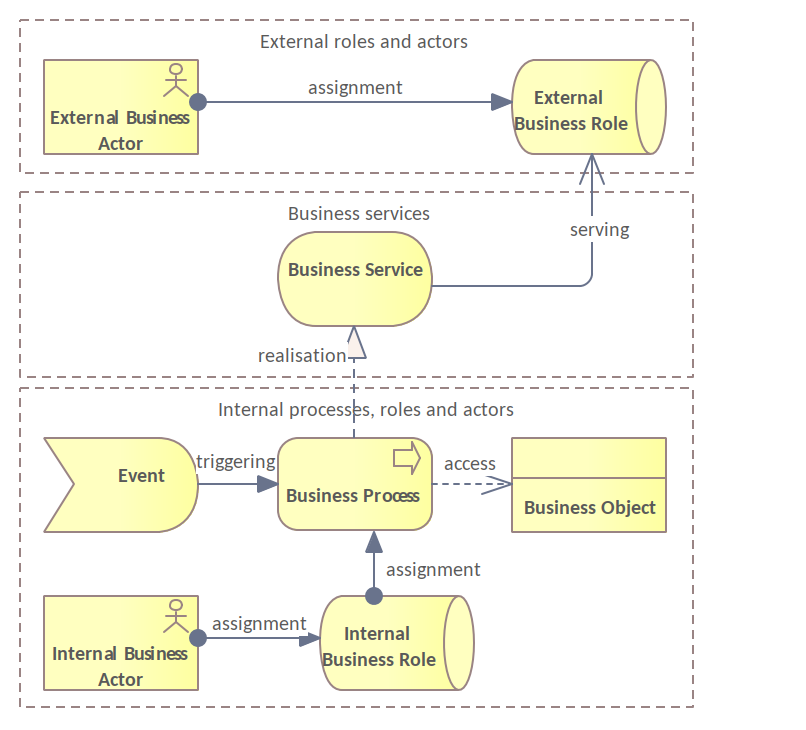
\includegraphics[width=0.4\textwidth]{images/views/Business view.png}
%		\caption{The prototypical business structure view}
%		\label{fig:business-structure-protopypical}
%	\end{wrapfigure}
	
	\begin{figure}[h]
		\centering
		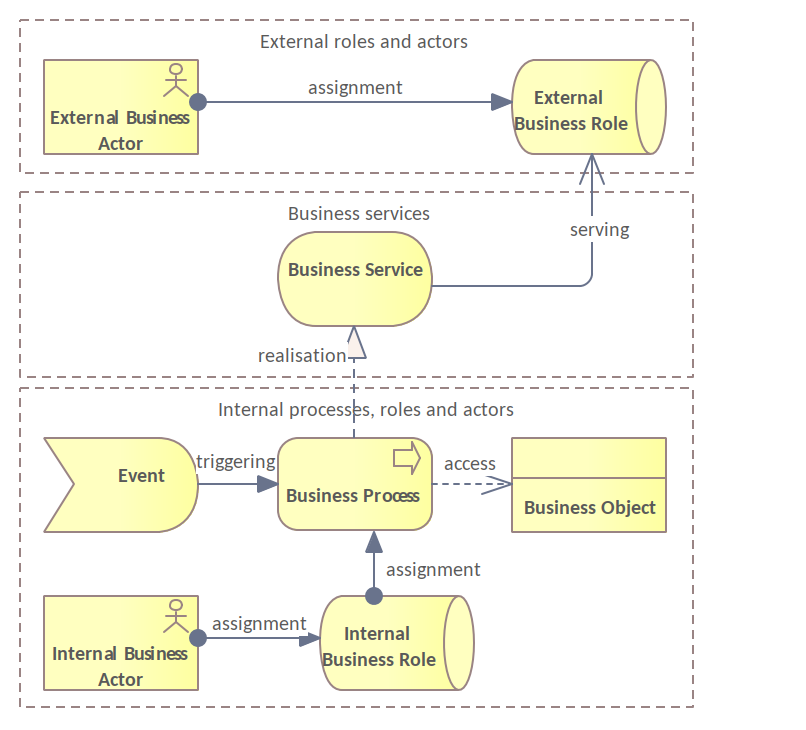
\includegraphics[width=0.4\textwidth]{images/views/Business view.png}
		\caption{The prototypical business structure view}
		\label{fig:business-structure-protopypical}
	\end{figure} 
	
	The topmost layer accounts for the external players or \textit{actors}, which represent a business entity that is capable of performing behaviour and \textit{roles}, which represent skills and responsibilities for performing specific behaviour, and to which an actor can be assigned \citep{archimate3.1}. 
	
	The middle layer represents the \textit{services} that are offered by the organisation to external players. A business service represents explicitly-defined behaviour that a business role, business actor or business collaboration exposes to its environment \citep{archimate3.1}.
	

	
	The lower layers accounts for the internal organisation in terms of \textit{events}, \textit{roles}, \textit{processes} and \textit{objects}. The business process represents a sequence of business behaviours that achieves a specific result such as a defined set of products or business services. The business event represents an organisational state change; while a business object represents a (passive) concept used within a particular business domain.
	

	\subsection{Current asset life-cycle stages}
	\label{sec:lifecycle-current-stages}
	
	The current asset life-cycle process is organised in six stages: \textit{inception (or evolution)}, \textit{implementation}, \textit{pre-release}, \textit{release}, \textit{publication} and \textit{consumption}. Each of the stages represents a business sub-process. Figure \ref{fig:lifecycle-current-stages} depicts the order in which stages flow and indicates that each stage process accesses a data asset, the central artefact in the diagram.
	
	\begin{figure}[h]
		\centering
		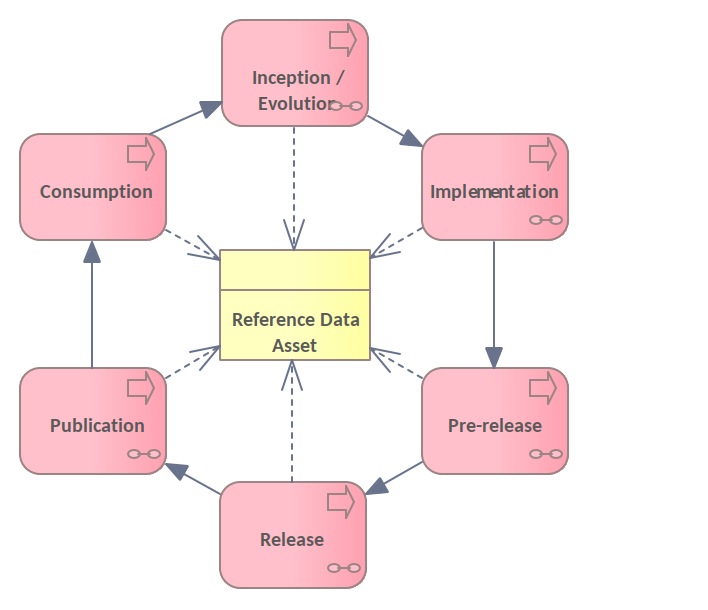
\includegraphics[width=0.5\textwidth]{images/business/Lifecycle process only (current).png}
		\caption{The current asset lifecycle stages}
		\label{fig:lifecycle-current-stages}
	\end{figure} 

	The \textit{inception} stage means that a request arrives for creating and publishing a new data asset and it is being dealt with by the team. The \textit{evolution} stage is similar, only that the request is one for change of an existing data asset. There is no difference in the way these two requests are treated and so the stage name is a conflation of the two. This stage also includes negotiating the request back with the client and then finally deciding and planning its implementation and publication. 
	
	The \textit{implementation} stage deals with actually changing, authoring, converting (MS Excel to XML and back) and verifying the client request. 
	
	\textit{Pre-release} marks that the content has been implemented accordingly and can be validated by a second pair of eyes implementing the \textit{four eyes principle} implemented in SU. This verification and validation is performed by checking the validation reports and by comparing the difference between current and previous versions of the asset conveyed in a diff report. 
	
	In the \textit{release} stage the validated content is placed in a dedicated location of the common repository which indicates that the content is fit for publication. 
	
	The \textit{publication} stage deals with packaging the content and disseminating it to the selected data disseminators, Cellar being the most important. During this stage, a set of announcements and communications ensure that the main stakeholders and the broad public are aware of the published new version of the asset. 
	
	\textit{Consumption} stage is the one that happens outside SU borders. It is clients who use the data and then, in the process, come up with additional requests for either changing existent assets or adding and publishing new ones. 
	
	\subsection{Actors and roles}
	\label{sec:lifecycle-roles}	
	
	This section describes identified actors and roles relevant to the asset life-cycle process. Figure \ref{fig:internal-roles} depicts their relations.
		
	\textit{Asset manager} (a mix of \textit{operational and business data steward}) is primarily responsible for data content, context and associated business rules. This role is characterised by full responsibility for the asset quality, enforcing policies and data governance processes, and ensuring asset fitness (both content and metadata) to business needs. In the SU, this role is also responsible for high-level interaction with main stakeholders and important clients.
	
	\textit{Team steering committee} (also known as the team meetings) is a body composed of business, technical and analytical roles whose main purpose is to provide executive and operational guidance validating business requests and assessing both data management and broader impact, determining implementation priority, as well as promoting data governance and standardisation practices.
	
%	\begin{figure}[h]
%		\centering
%		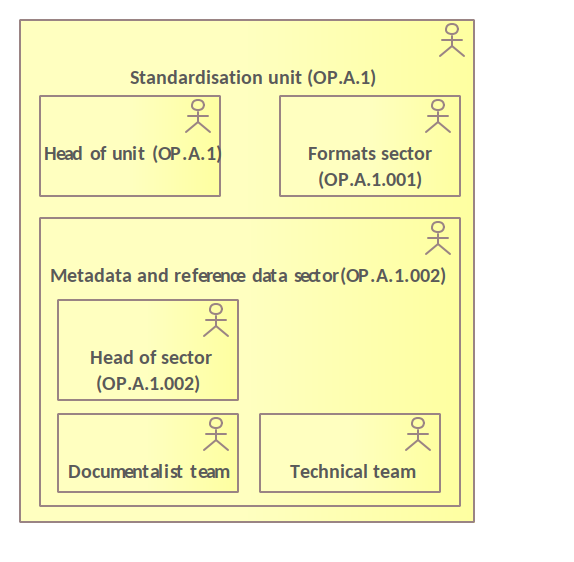
\includegraphics[width=0.47\textwidth]{images/business/Internal Business Actors.png}
%		\caption{The actors in metadata and reference data sector}
%		\label{fig:actors-team}
%	\end{figure} 
	
	\begin{figure}[h]
		\centering
		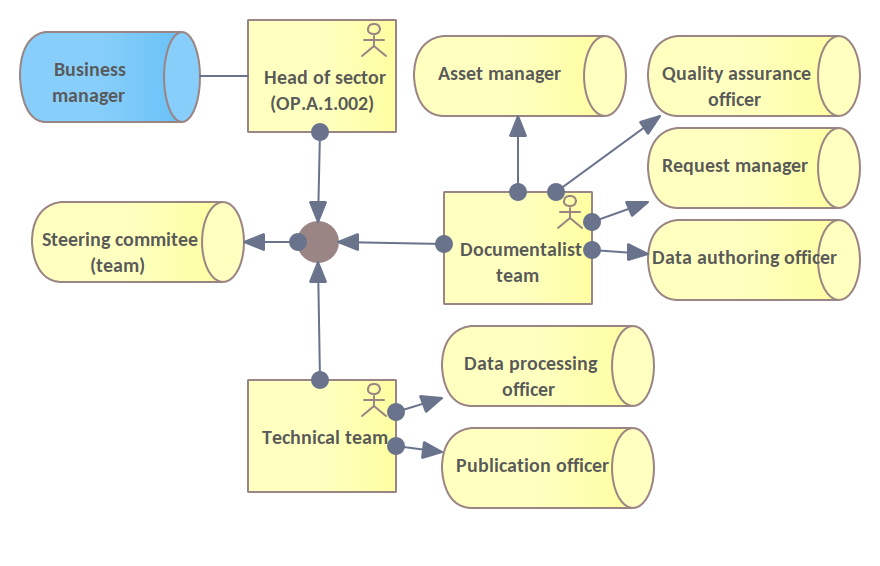
\includegraphics[width=0.7\textwidth]{images/business/Internal Roles.png}
		\caption{The internal roles in metadata and reference data sector}
		\label{fig:internal-roles}
	\end{figure}
	
	\textit{Request manager} is the interface with the client collecting change requests, assessing business needs and translating them into data management requirements, all being summarised and documented case-by-case. 
	
	\textit{Data authoring officer} is responsible for editing data in a content management system implementing the cases prepared by the request manager.
	Quality assurance officers validate that the content implementation is correct from both technical and business points of view. 
	
	\textit{Data processing officer} is a technical role that is responsible for preparing the assets for publication. The responsibilities include, but are not limited to, data storage, manipulation, automatic transformation and generation of validation and assessment reports. 
	
	\textit{Publication officer} is a technical role responsible for packaging and disseminating assets to specialised platforms.
	
	\textit{Stakeholder steering committee} is a body representing the main clients and stakeholders ensuring data and model harmonisation, alignment of data management practices and adoption of international standards.
	
	\textit{Client} (\textit{change requester} and \textit{data user}) is a generic external role who, on one side, consumes data and services provided by the Standardisation Unit and, on the other side, suggests publication of new assets or modification of existing ones. 
	
	\textit{Data disseminator} is an external role providing the Standardisation Unit with reliable data dissemination capabilities which are meant to make assets available for clients.

	The external roles and stakeholders have already been addressed in the motivations structure depicted in Figure \ref{fig:stakehodlers-roles}. Each of these roles has a corresponding element in the business model and will be employed accordingly.

	\subsection{Current asset life-cycle overview}
	\label{sec:lifecycle-current}
	
	This section assembles the asset life-cycle process stages and the main internal roles together into an overview diagram depicted in Figure \ref{fig:lifecycle-current}. It indicates what roles are assigned to which processes, along with a cyclical depiction of the process sequence. Next we comment on the involvement of each role in the asset life-cycle process. All the life-cycle stages are internal to the SU except for the last one, consumption, which takes place at the client's premises.
	
	\begin{figure}[h]
		\centering
		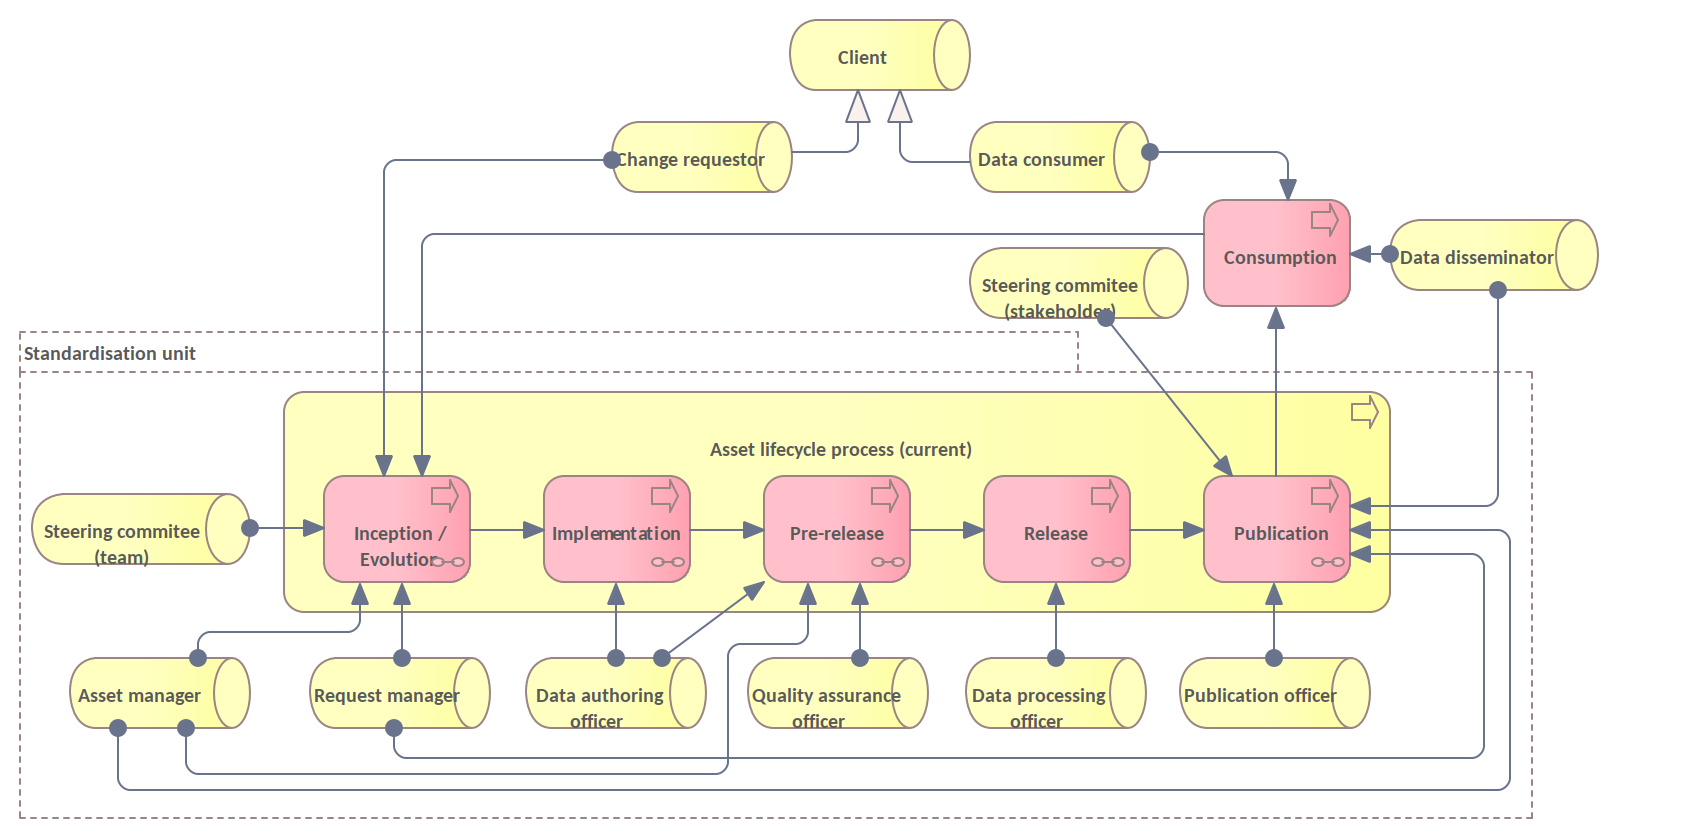
\includegraphics[width=1.05\textwidth]{images/business/Lifecycle (current).png}
		\caption{The current asset lifecycle stages and roles}
		\label{fig:lifecycle-current}
	\end{figure} 
	
	In the inception/evolution stage, the request manager is responsible for creating, documenting and ensuring descriptive completeness for requests arriving from clients to change existing assess or to create new ones. These requests are managed as individual or, on some occasions, interdependent cases. This role serves as the primary interface with third parties. For this reason, in the publication stage, this role communicates with stakeholders and broad public about asset changes when they are published.
	
	The asset manager is in charge of analysing and summarising the request case in the inception/evolution stage. This role intervenes in the pre-release stage to acknowledge that the case has been implemented and the asset is fit for publication; then, in the publication stage, to check the impact assessment and release notes before they are used in the communication with external parties.
	
	The team steering committee is involved in the initial stage only. After a new change request case is created, the team steering committee decides whether the case shall be further processed and, if so, then the decision is about when and how.
	
	The data authoring officer is responsible for the case implementation and, in the pre-release stage, for verifying and validating their own work as the ``first pair of eyes'' (of the ``two pairs of eyes'' principle). The ``second pair of eyes'' verifying and validating the case implementation is enacted by the quality assurance officer in the same pre-release stage.
	
	Once the case is marked as fit for publication, in the release stage, it is placed automatically, or by intervention of the data processing officer, in a region of the common repository tagged for ``release''. If any technical issues are encountered, then the data processing officer intervenes and fixes them.
	
	In the publication stage, the publication officer generates the release artefacts and release notes, packages the assets and disseminates them to the dissemination partners. External steering committees, such as IMMC metadata sub-committee, GIL EuroVoc and others are asked for final feedback two weeks in advance before final dissemination.
	
	Next, we address the asset life-cycle stages in more detail as elicited from the technical and business teams of the SU. These descriptions are not covering ultimate details of the process, but aim at describing the important building blocks of the current stages. 
	
	\subsection{Current inception and evolution stage}
	\label{sec:inception-current}
	
	\begin{figure}[h]
		\centering
		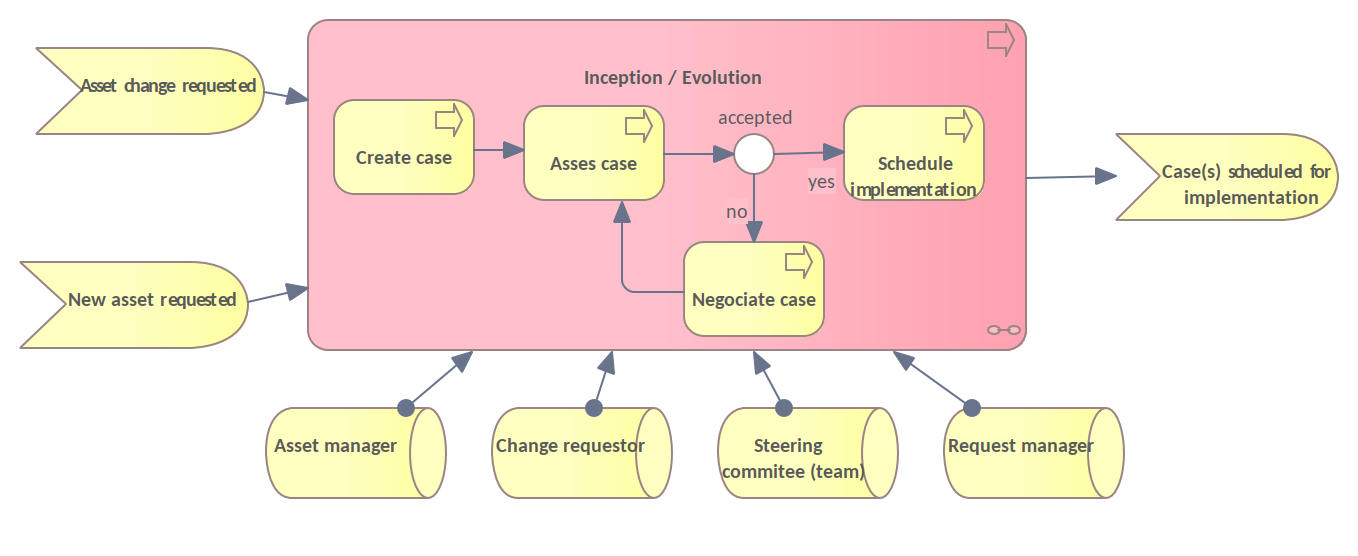
\includegraphics[width=.8\textwidth]{images/business/current/InceptionEvolution.png}
		\caption{The current process for the inception and evolution stage}
		\label{fig:evolution-current}
	\end{figure}		
	
	The process, depicted in Figure \ref{fig:evolution-current}, starts when a client request arrives to either update a data asset or create a new one. This case, after being recorded, analysed and summarised, is assessed by the asset manager and then discussed in the team meeting. 
	
	
	When the case is accepted, then it is scheduled for implementation. Otherwise, i.e. when it is not (initially) accepted, the case enters a ``negotiation'' stage, due to one of two things: either the case is incomplete and more information is required from the client, or the case is unacceptable and a rejection is provided to the client with an explanation of why or possibly even with suggestions / counter-proposals. 
	
	Client communication is mainly carried out by email or by telephone, with the cases being managed using the Jira ticket management system \citep{jira}. 
	
	The process ends when either the case is rejected or when it is scheduled for implementation. 

	
	\subsection{Current implementation stage}
	\label{sec:implementation-current}
		
	Figure \ref{fig:implementation-current} depicts the current implementation process. It starts when the case is queued for implementation. The data authoring officer modifies the asset content according to the instructions provided in the case description. The editing takes place in an MS Excel \citep{excel} workbook which represents an interface to the asset content. MS Excel is the main editing tool. Once the changes are complete, the workbook is committed into the SVN repository \citep{svn}, which triggers an automatic conversion of the MS Excel workbook into an XML form \cite{xml11-spec}. The XML form is considered the primary asset source structured with CAT-XSD scheme, and for this reason, sometimes we call it ``CAT-XML''. It is further converted back into MS Excel workbook form, this way entering a conversion loop which also serves as validation mechanism ($XML \rightarrow Excel \rightarrow XML \rightarrow Excel$).
	
	\begin{figure}[h]
		\centering
		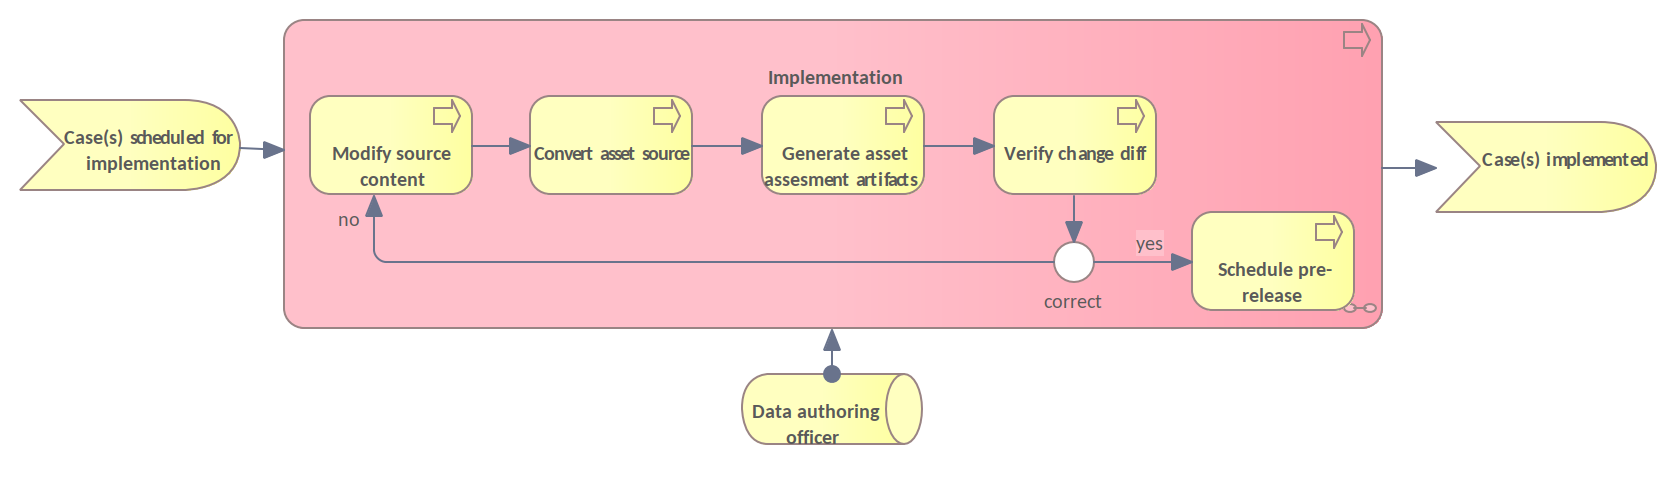
\includegraphics[width=.9\textwidth]{images/business/current/Implementation.png}
		\caption{The current process for the implementation stage}
		\label{fig:implementation-current}
	\end{figure}
	
	Once the asset is converted into XML form, it becomes possible through a set of Perl scripts and XSLT style-sheets \citep{xslt3-Kay} to automatically generate assessment artefacts such as the diff report and the schema validation report. The diff report indicates what changes have been done to the content between the previous and the most recent versions, while the validation report details violations, if any, of XML structural constraints.
	
	The editor then verifies the diff report to ensure the case implementation completeness and that the asset can be tagged for pre-release. Otherwise, the content should be edited once again. 
	
	The process ends with the asset being marked for pre-release, which means that the case implementation is complete.
	
	\subsection{Current pre-release stage}
	\label{sec:pre-release-current}	

	The pre-release stage is depicted in Figure \ref{fig:pre-release-current}. Once the case is marked ``implemented'', and the assessment artefacts were generated after the conversion into XML form, the second verification and validation can be performed by the quality assurance officer. 
	
	\begin{figure}[h]
		\centering
		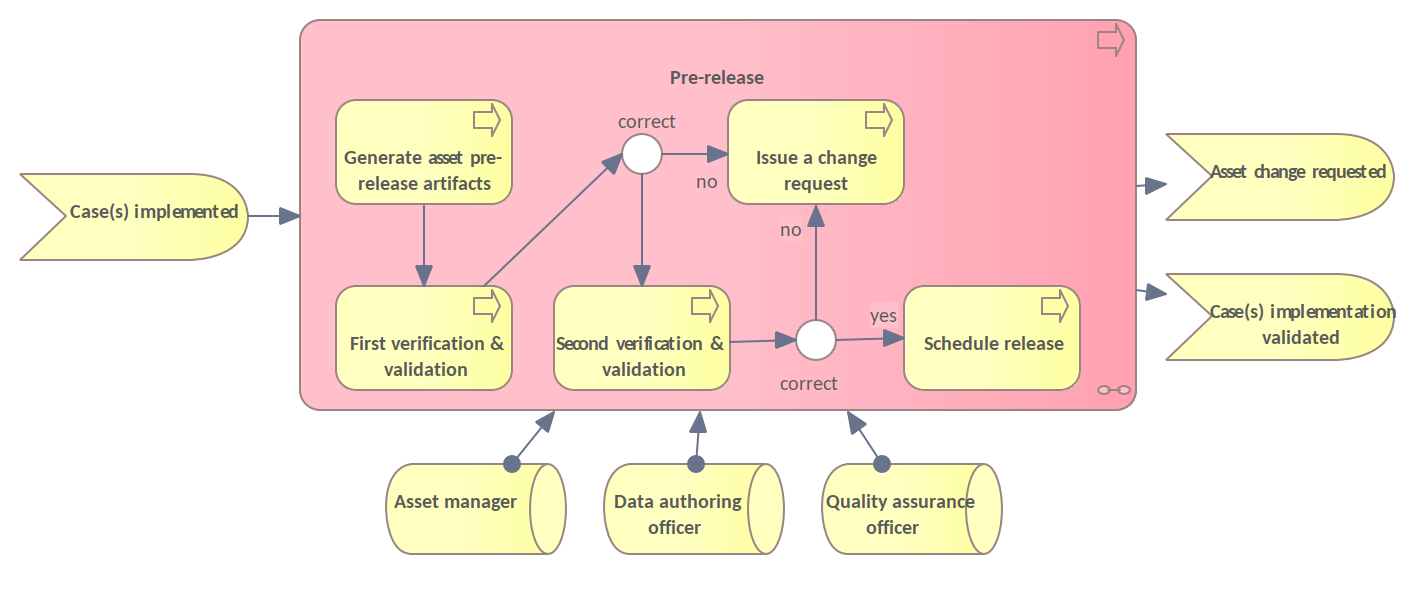
\includegraphics[width=.65\textwidth]{images/business/current/Pre-release.png}
		\caption{The current process for the pre-release stage}
		\label{fig:pre-release-current}
	\end{figure}

	If issues are identified in the case implementation, the quality assurance officer creates a new request for changes and the case returns to the implementation stage; otherwise, the case implementation is validated and the asset is marked as ready for release. 
	
	This process involves mostly manual steps. Some minor content transformation can take place such as improving the serialisation of RDF files (called internally as RDF ``prettification''), as well as an additional validation of record identifiers in the XML file. These operations, however, are merely technicalities and do no have any business relevance. Therefore they are omitted in the process diagram from Figure \ref{fig:pre-release-current}. 

	\subsection{Current release stage}
	\label{sec:release-current}
	
	\begin{figure}[h]
		\centering
		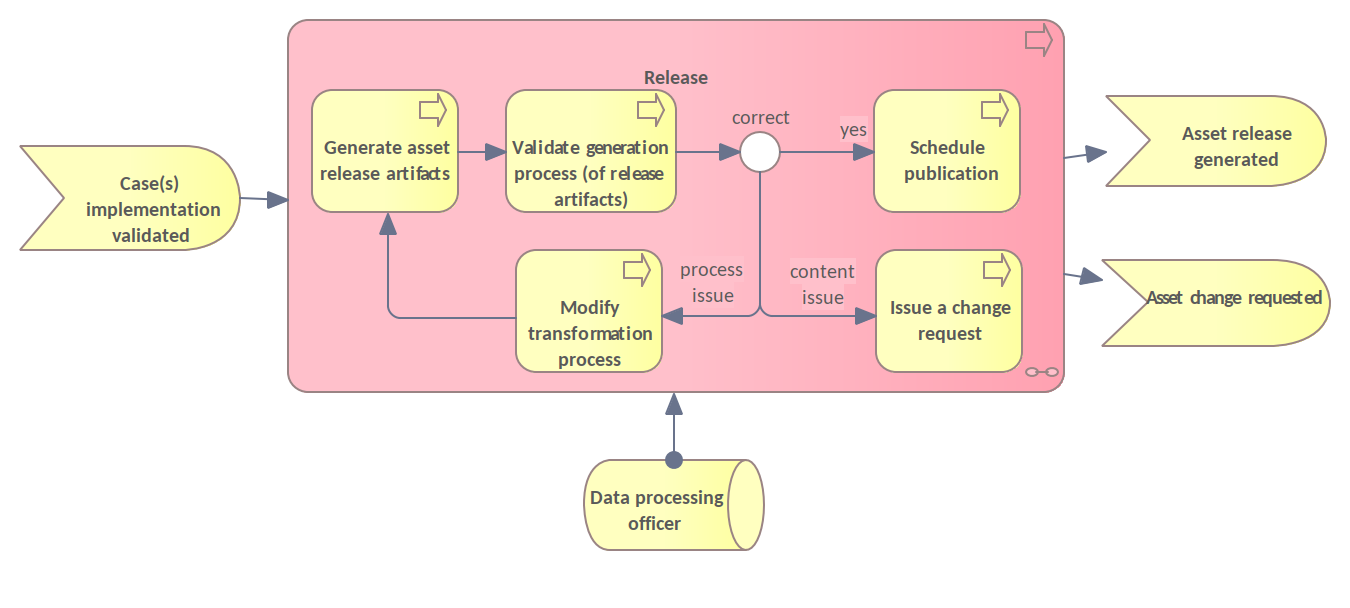
\includegraphics[width=.6\textwidth]{images/business/current/Release.png}
		\caption{The current process for the release stage}
		\label{fig:release-current}
	\end{figure}

	The release stage is a symbolic step after an asset has been verified and validated by four ``pairs of eyes'' and it has been confirmed that all cases have been correctly implemented, also that the asset is fit for release in the subsequent publication. This is depicted in Figure \ref{fig:release-current}.

	The release stage is realised by copying the updated version of the asset into a special area of the common repository and marked with the ``release'' tag.

	\subsection{Current publication stage}
	
	The current publication stage is depicted in Figure \ref{fig:publication-current}. It is a wide-ranging process that involves almost all the various roles. 
	
	\label{sec:publication-current}
		\begin{figure}[h]
		\centering
		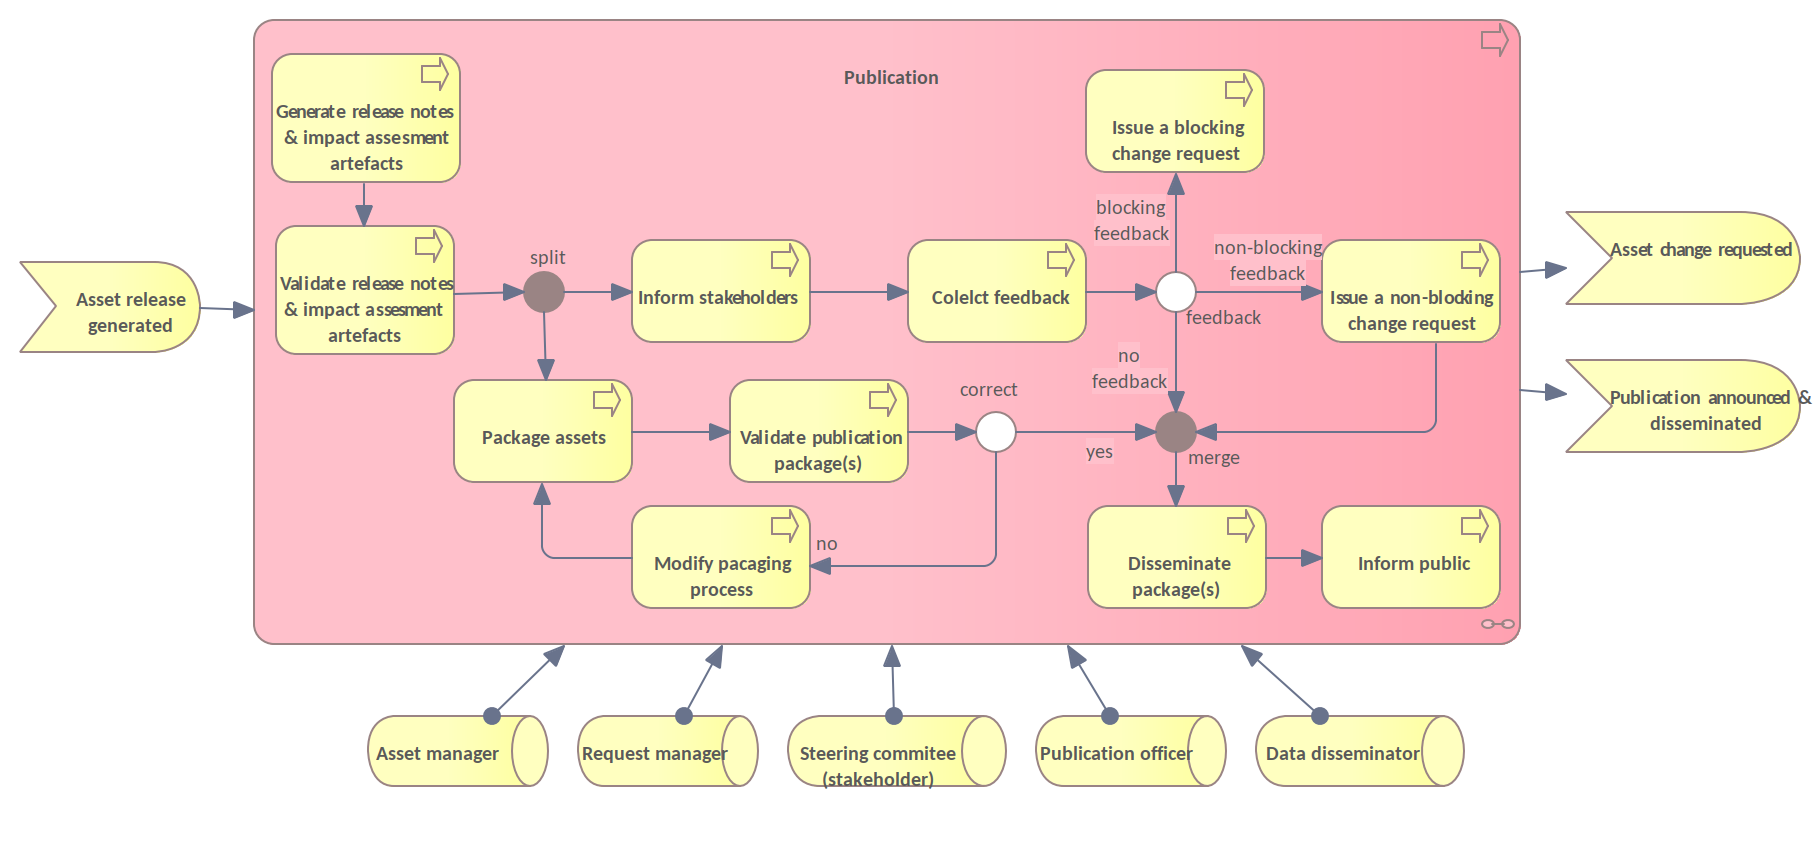
\includegraphics[width=1.03\textwidth]{images/business/current/Publication.png}
		\caption{The current process for the publication stage}
		\label{fig:publication-current}
	\end{figure}

	The publication process starts several weeks before the scheduled publication date, when a code freeze is announced and all pre-selected assets are marked for release. It commences by generating (from the CAT-XML source) a selection of forms and formats to ease asset consumption by various clients. Mostly XSD, CAT-XML and SKOS-AP-EU forms are generated that are serialised in XML, Turtle and JSON formats. In addition, some assets are also prepared in Genericode, MS Excel/CSV, MarcXML, GeoJSON and other formats. 
	
	Next, the publication notes are prepared together with a few different impact assessments specially prepared for targeted stakeholders. These communication artefacts are checked for correctness and sent to the corresponding stakeholders. After a predefined number of days (usually two weeks) the feedback, if any, is collected. Reception of no feedback is considered as a tacit acceptance of the current publication and that the process can continue. Seldom is blocking / non-blocking feedback received which leads to creation of new change requests and, depending on the situation, last-minute changes are executed. On the other hand, if the feedback received is non-blocking, the intervention is scheduled for the next publication. 
	
	In parallel, a packaging process is executed during which the assets are prepared for dissemination. They are assembled in packages accompanied by their content-related and technical metadata, user manuals, format documentation and, of course, the asset itself expressed in all pre-generated forms and formats, the release artefacts. The packages are verified to establish if they can be accepted by the target dissemination platforms.
	
	Finally, the packages are disseminated and the successful publication is announced to the broad public. The dissemination is done primarily through Cellar\citep{cdm-francesconi2015ontology}, although other dissemination channels are also employed, among which are Wikidata\citep{vrandevcic2014wikidata}, Publications Office Open Data Portal (ODP), Bartoc \citep{ledl2016describing}, JoinUp platform \citep{hillenius2013free}.
	
	This section completes the detailed presentation of the asset life-cycle process as it is today. 
	
	The digital transformation currently undertaken by SU management, that is in part targeted by this architecture, has an impact on the asset life-cycle business, application and technical architectures. The next sections describe how the new asset life-cycle architecture is envisaged. 
		
	\subsection{New asset life-cycle overview}
	\label{sec:lifecycle-new}	
	
	The structure of the new asset life-cycle process is depicted in Figure \ref{fig:lifecycle-new}. In this new architecture, we propose incremental changes, so as to cause minimal disruption to the team and ongoing operations. 

	\begin{figure}[h]
		\centering
		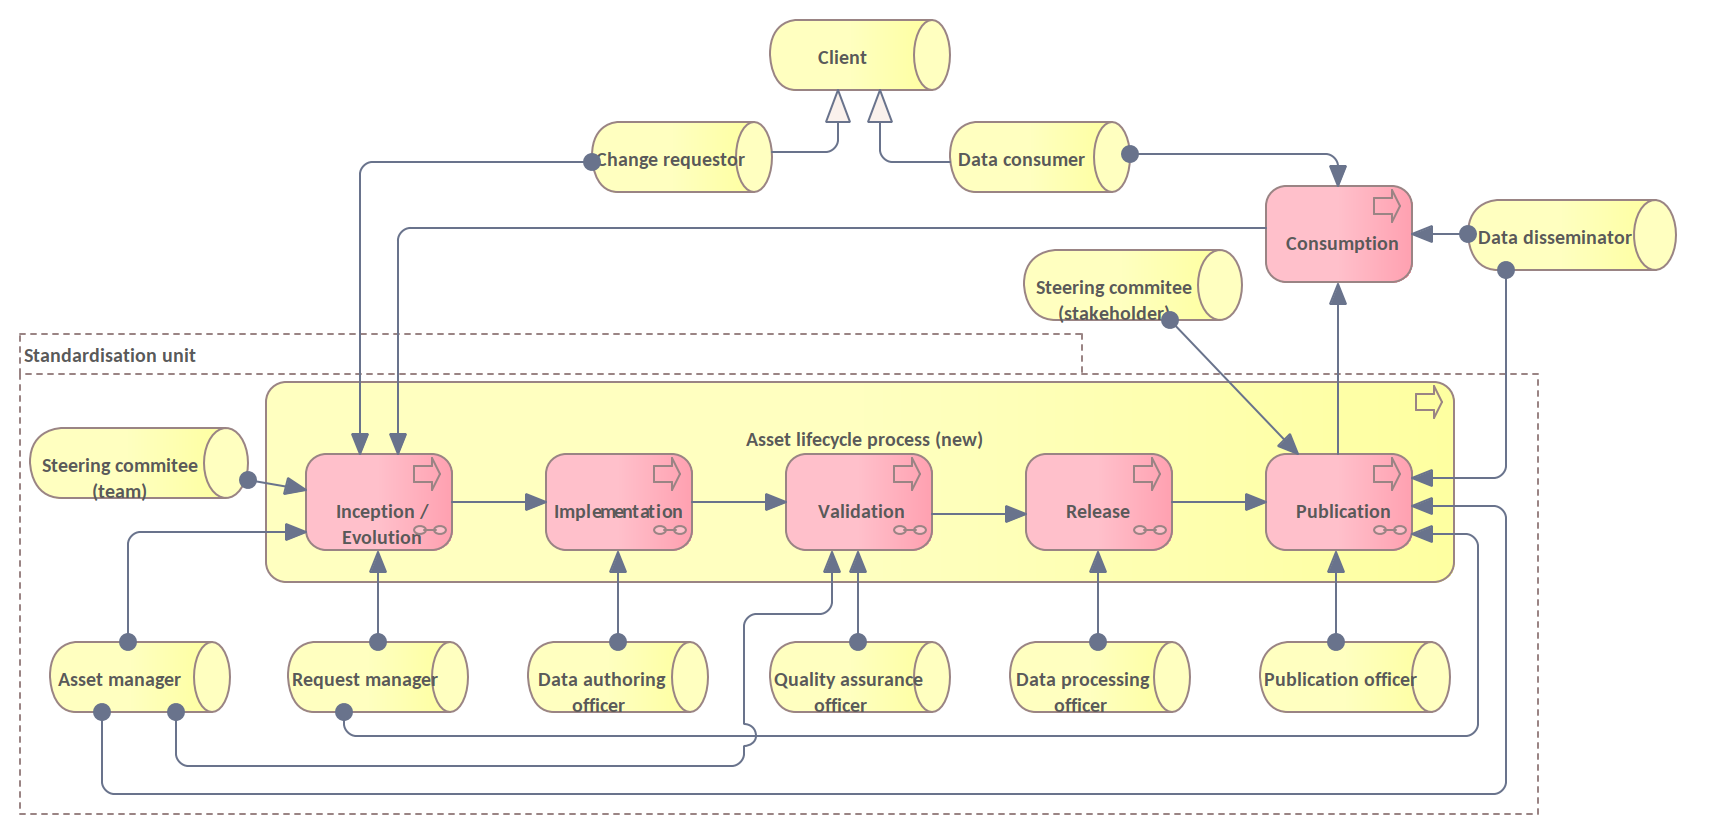
\includegraphics[width=1.05\textwidth]{images/business/Lifecycle (new).png}
		\caption{The current asset life-cycle stages and roles}
		\label{fig:lifecycle-new}
	\end{figure}
	
	This process is similar, in structure and stage names, to the current one: i.e. six stages are circularly linked. The only difference is the replacement of the pre-release stage by a validation stage. There are, however, significant changes in the structure of three stages: implementation, validation and release, while the inception/evolution stage is identical to the current one, and the publication stage is almost entirely unchanged. These changes are addressed in detail in the following sections.
		
	There are no new roles in the new process; however, there is a difference in the role allocation and involvement (of the various roles) at different stages of the process compared to the current one. 
	
	As mentioned above, the implementation/evolution stage is identical to the current one. So, after the case has been registered and processed, the implementation is scheduled. How it happens in the new workflow is presented in the next section. 
			
	\subsection{New implementation stage}
	\label{sec:implementation-new}

	The new implementation process is depicted in Figure \ref{fig:validation-new}. The main digital transformation at this stage is adoption of the RDF asset source, and the switch from MS Excel as the content editor to VocBench3 \citep{stellato2017towards,stellatovocbench} semantic web editor. 
	
	\begin{figure}[h]
		\centering
		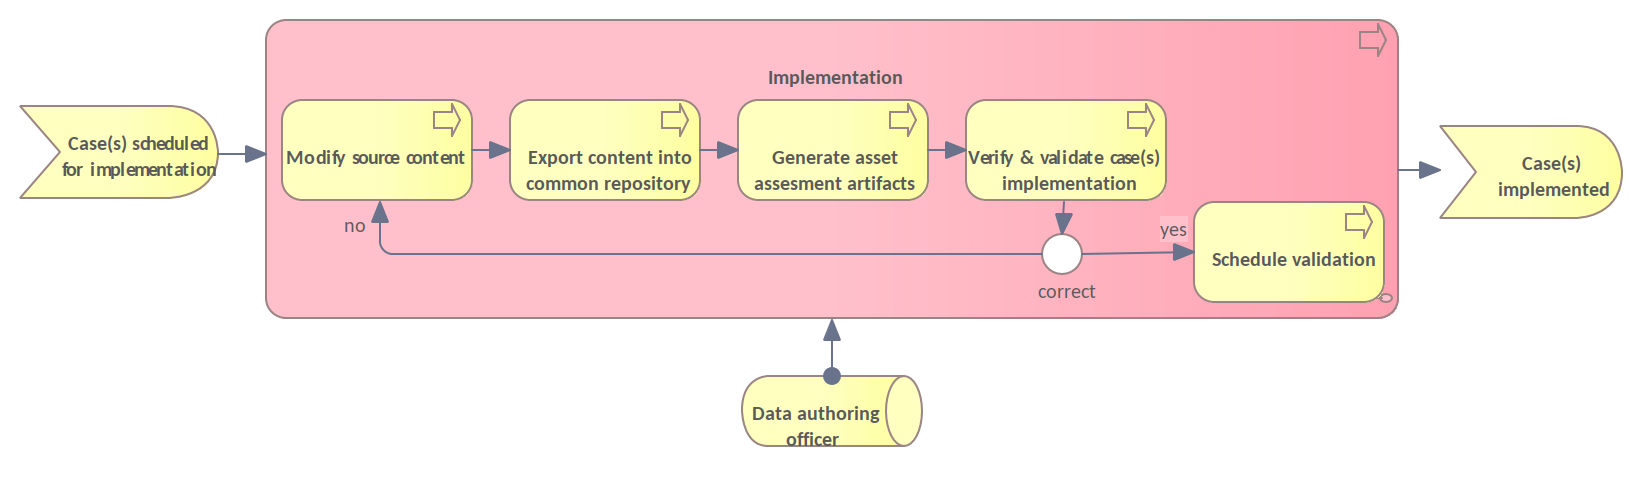
\includegraphics[width=1.05\textwidth]{images/business/new/Implementation.png}
		\caption{The new process for the implementation stage}
		\label{fig:implementation-new}
	\end{figure} 

	The overall process looks very similar to the current one; however, the employed technology for the source editing, i.e. VocBench3 \citep{stellatovocbench} and SKOS model(s) \citep{skos-spec}, render an entirely different editing experience when modifying the source content to implement the request case.
	
	When the editing is complete, the content is exported from VocBench into the common repository and a set of asset assessment artefacts are generated. These artefacts include the asset diff report, the fingerprint report and the validation report (based on SHACL \citep{shacl-spec} validation rules). These reports are no longer implemented based on XSLT technology \citep{xslt3-Kay}, because the underlying source is the new RDF representation \citep{rdf11} and no longer (CAT-)XML. More technical details are addressed in the application architecture in Section \ref{sec:implementation-application}.
	
	The editor (data authoring officer) then verifies that the case is implemented correctly and, if so, then validation is scheduled to be undertaken by the quality assurance office. Otherwise, if some issues are detected, then more editing is performed in VocBench3.
		
	
	\subsection{New validation stage}
	\label{sec:validation-new}	
	
	The validation stage is new in the asset life-cycle process. Here, the correctness assessment is separated into two steps: verification and validation. This is a continuation of the current conception of how the case implementation is being assessed. The verification primarily focuses on the business aspects of the case implementation, whereas the validation deals with  technical and more formal aspects of the content structure and consistency. As the new technology allows for semantic accounts, then validation also extends to deal with semantics. 	 

	\begin{figure}[h]
		\centering
		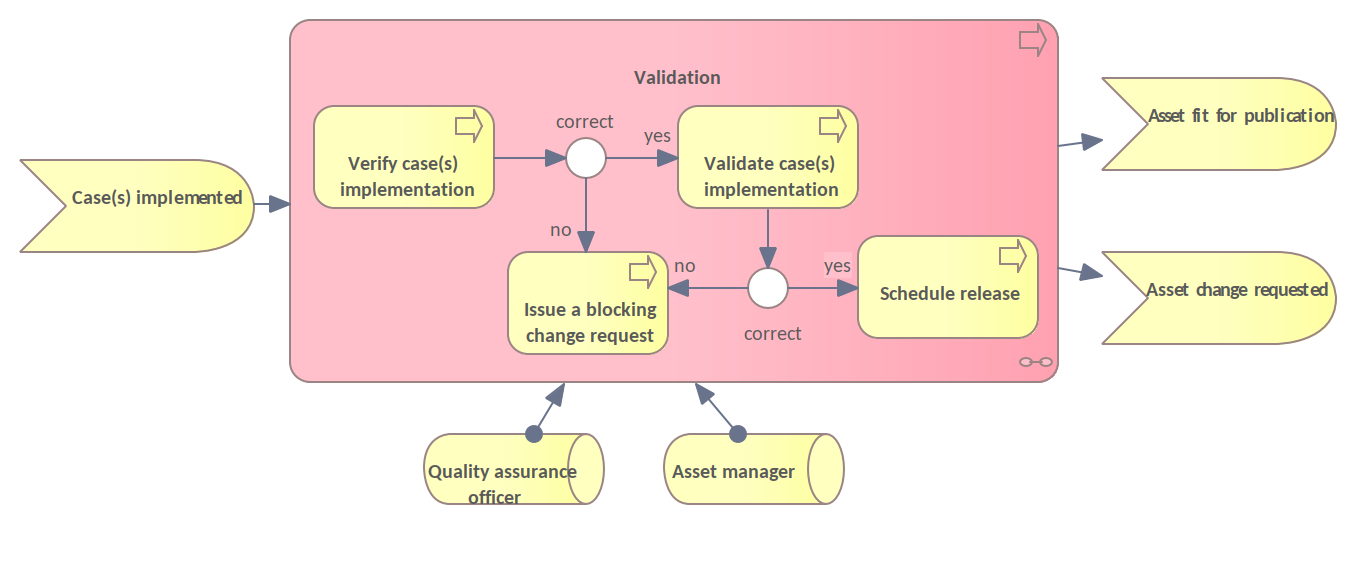
\includegraphics[width=.892\textwidth]{images/business/new/Validation.png}
		\caption{The new process for the validation stage}
		\label{fig:validation-new}
	\end{figure}

	In case errors are detected in the implementation, the quality assurance officer issues a  change request and the case goes back into the implementation stage. Otherwise, the case implementation is considered correct and, from then on, a release can be scheduled. This is performed by the asset manager. 
		
	\subsection{New release stage}
	\label{sec:release-new}
	
	The new release stage, depicted in Figure \ref{fig:release-new}, differs considerably from the current one. This stage is no longer one of simply marking the asset implementation as ``fit for publication'', but deals with all data transformations and preparation of artefacts necessary in the publication stage.
	
	\begin{figure}[h]
		\centering
		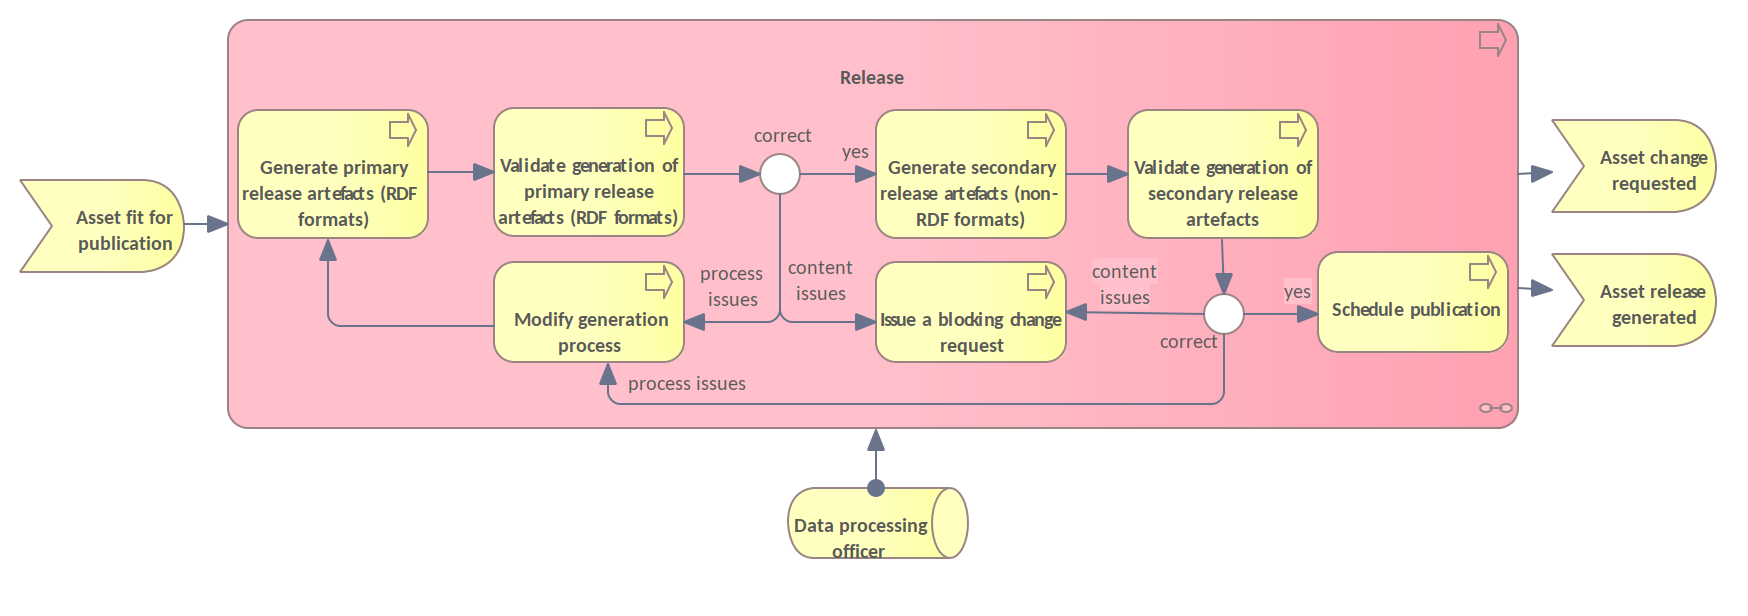
\includegraphics[width=1.05\textwidth]{images/business/new/Release.png}
		\caption{The new process for the release stage}
		\label{fig:release-new}
	\end{figure}

	The release starts when all change request cases, in the scope of the scheduled publication, have been implemented and validated. Then, the primary release artefacts are generated from the RDF source is expressed in SRC-AP form \citep{src-ap-vb3}. The main artefacts are the source in SKOS-AP-EU form \citep{skos-ap-eu}, a special extension of the SKOS-AP-EU which is necessary for publishing the content in Cellar because of backward compatibility issues (called SKOS-AP-EU-Act), and the SKOS core \citep{skos-spec} representation. These artefacts are also generated in RDF/XML \citep{rdf-xml-Schreiber:14:RXS,rdf-xml-Beckett:04:RSS}, Turtle \citep{turtle-Carothers:14:RT} and JSON-LD \citep{sporny2014json,spornyjson} formats. 
	
	The transformation process is accompanied by a set of validation processes meant to safeguard the output and ensure that the transformations are executed correctly. The validation reports are checked by the data processing officer. If process-related issues are detected, then most likely the processes contain bugs and need to be fixed. If content related issues are spotted, then a new change request is created and the process reverts to the implementation stage. 
	
	After primary release artefacts are created, then secondary release artefacts are created. All of them are non-RDF forms that are currently produced for clients (CAT-XML, XSD, Genericode, MS Excel/CSV, MarcXML, GeoJSON, etc.) and must continue so. An automated validation of the generated assets, to the greatest extent possible, secures and ensures quality of the output. As in the case of primary artefacts, if errors are detected then depending on their nature, either the data transformation process must be updated or a content change request is issued and the process reverts to the implementation stage. 
	
	The transformation technology employed here needs to provide ETL\footnote{Extract, transform, load (ETL) is the general procedure of copying data from one or more sources into a destination system which represents the data differently from the source(s) or in a different context than the source(s).}/ELT\footnote{Extract, load, transform (ELT) is a variant of ETL where the extracted data is loaded into the target system first.}-like capabilities for both RDF and data formats. An extended discussion about application capabilities is covered in Section \ref{sec:release-application}.
	
	At the end of this stage, all important asset transformations and data conversions must be complete and the necessary forms and formats consumed by target clients shall be available for publication. Finally, assets are copied into the special place within the common repository available to the publication process. 
	
	\subsection{New publication stage}
	\label{sec:publication-new}
	
	The new publication stage process is depicted in Figure \ref{fig:publication-new}. This process is very similar to the one currently performed and that is described in Section \ref{sec:publication-current}.
	
	\begin{figure}[h]
		\centering
		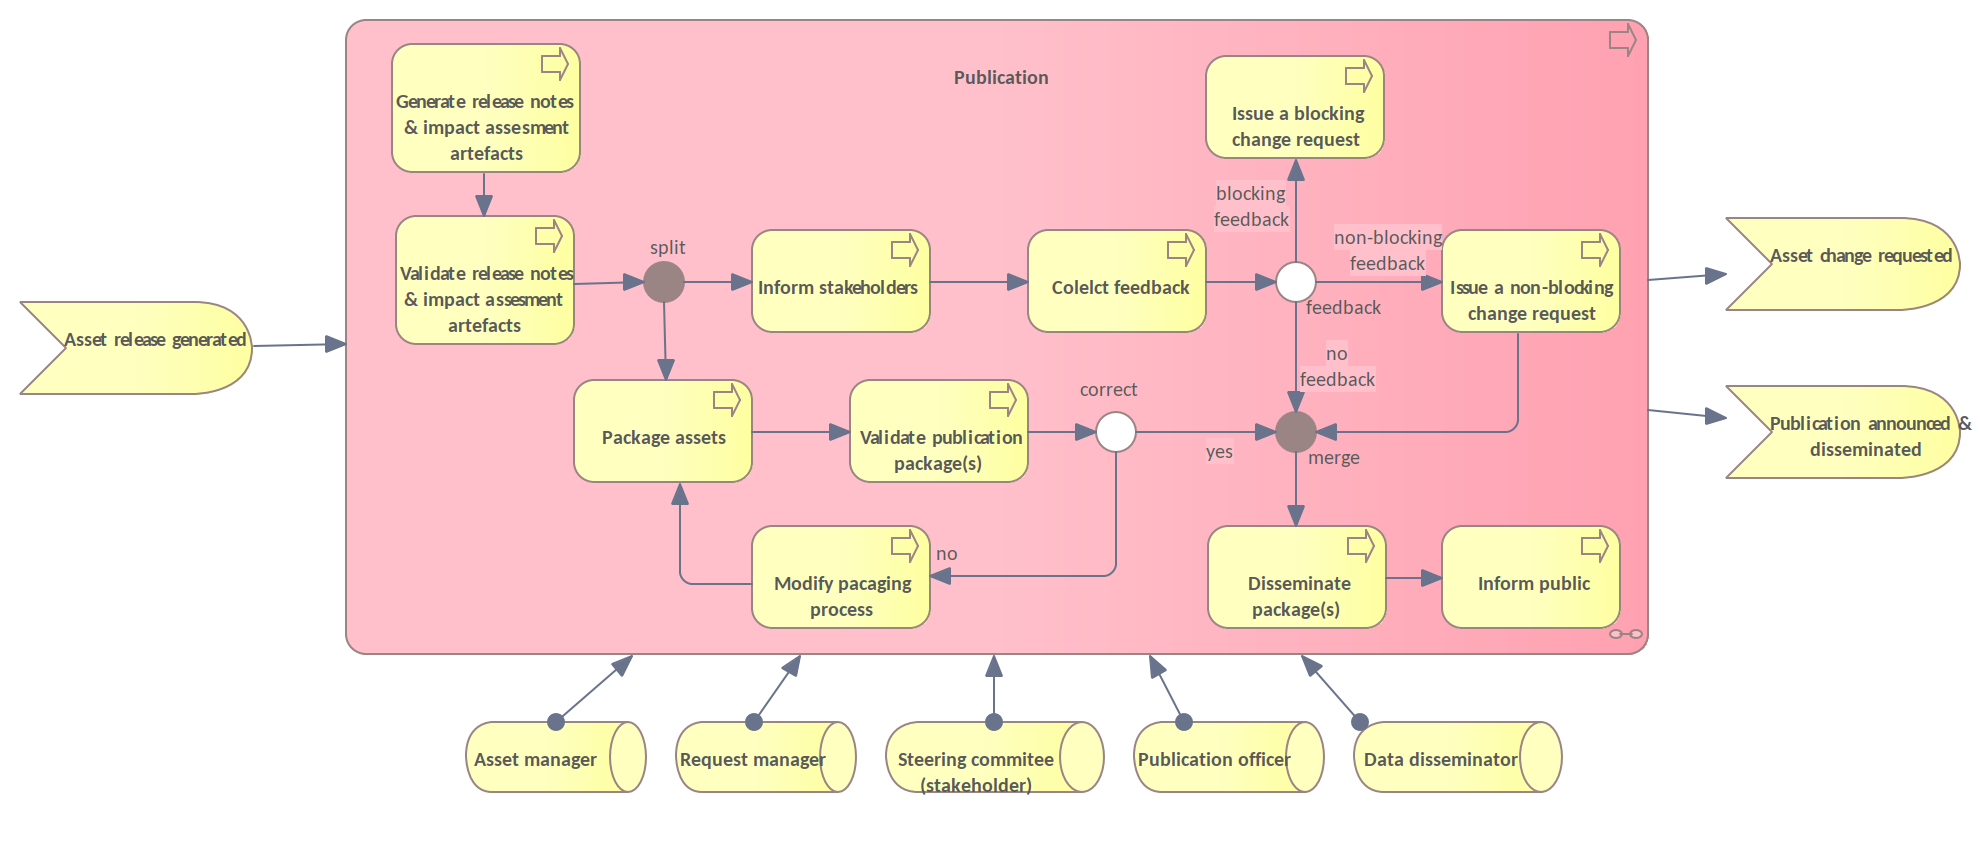
\includegraphics[width=1.05\textwidth]{images/business/new/Publication.png}
		\caption{The new process for the release stage}
		\label{fig:publication-new}
	\end{figure}

	The main difference in this process is the starting point. If currently it starts by transforming and converting the asset source into all forms and formats demanded by clients, then the new process starts from the premise that the entire publication content has already been generated. 
	
	The new process starts by the generation of release notes and set of impact assessment reports destined for different stakeholders. These communication artefacts are verified by the asset manager and then the request manager disseminates the news to the stakeholders and the broad public about the upcoming publication. The stakeholders may have a veto or comment on the current publication, just as is currently foreseen.   
	
	What is left, at this stage, from the technical point of view, is packaging and distributing the publication packages to the data disseminators. The process ends when the latest version of published assets are accessible via the selected data disseminators and the broad public is informed. 
	
	This section finishes the description of the business architecture. Next is presented the application architecture accounting for necessary services and capabilities that must be in place to serve the current business processes along with an account of what components realise such services. 
	